\documentclass[]{article}
\usepackage{lmodern}
\usepackage{graphicx}
\usepackage{adjustbox}
\usepackage{amssymb,amsmath}
\usepackage{ifxetex,ifluatex}
\usepackage{listings}
\usepackage[T1]{fontenc}
\usepackage[utf8]{inputenc}
\usepackage{microtype}
\usepackage[margin=1in]{geometry}
\usepackage{hyperref}
\usepackage{framed}
\usepackage{graphicx,grffile}
\usepackage{fancyvrb}
\usepackage{multirow}
\usepackage{subfig}
\makeatletter
\def\maxwidth{\ifdim\Gin@nat@width>\linewidth\linewidth\else\Gin@nat@width\fi}
\def\maxheight{\ifdim\Gin@nat@height>\textheight\textheight\else\Gin@nat@height\fi}
\makeatother
% Scale images if necessary, so that they will not overflow the page
% margins by default, and it is still possible to overwrite the defaults
% using explicit options in \includegraphics[width, height, ...]{}
\setkeys{Gin}{width=\maxwidth,height=\maxheight,keepaspectratio}
\setlength{\parindent}{0pt}
\setlength{\parskip}{6pt plus 2pt minus 1pt}
\setlength{\emergencystretch}{3em}  % prevent overfull lines
\providecommand{\tightlist}{%
  \setlength{\itemsep}{0pt}\setlength{\parskip}{0pt}}

%%% Change title format to be more compact
\usepackage{titling}

% Create subtitle command for use in maketitle
\newcommand{\subtitle}[1]{
  \posttitle{
    \begin{center}\large#1\end{center}
    }
}

\setlength{\droptitle}{-2em}
  \title{MSAN 604 - Homework 3}
  \pretitle{\vspace{\droptitle}\centering\huge}
  \posttitle{\par}
  \author{Andre Guimaraes Duarte}
  \preauthor{\centering\large\emph}
  \postauthor{\par}
  \predate{\centering\large\emph}
  \postdate{\par}
  \date{December 6, 2016}
  
% Redefines (sub)paragraphs to behave more like section*s
\ifx\paragraph\undefined\else
\let\oldparagraph\paragraph
\renewcommand{\paragraph}[1]{\oldparagraph{#1}\mbox{}}
\fi
\ifx\subparagraph\undefined\else
\let\oldsubparagraph\subparagraph
\renewcommand{\subparagraph}[1]{\oldsubparagraph{#1}\mbox{}}
\fi

\usepackage{color}

%%%%%%%%%%%%%%%%%%%%%%%%%%%%%%%%%%%%%%%%%%%%%%%%%%%%%%%%%%%%%%%%%%%%%%%%%%%%%%%%%%%%%%%%%%%%%%%%%%%%%%%%%%%%%%%%%%%%%%%
\begin{document}
\null\hfill\begin{tabular}[t]{r@{}}
  \textbf{\LARGE Andre Guimaraes Duarte} \\
  \textbf{\Large 20406263}
\end{tabular}
%\maketitle

\begin{center}
\Huge
MSAN 604 - Homework 3

\Large
December 6, 2016

\normalsize
\end{center}

\section{Introduction}
Accurately forecasting time series data is important in many scenarios. For example, it can be used to predict import and export figures for a country given a prior history of this data. In this exercise, we model and forecast monthly Chinese export figures
(in 100 million USD). We have monthly import and export data from January 1984 to December 2008, as shown in Figures \ref{exports} and \ref{imports}.

\begin{figure}[!ht]
\centering
\begin{minipage}{.5\textwidth}
\centering
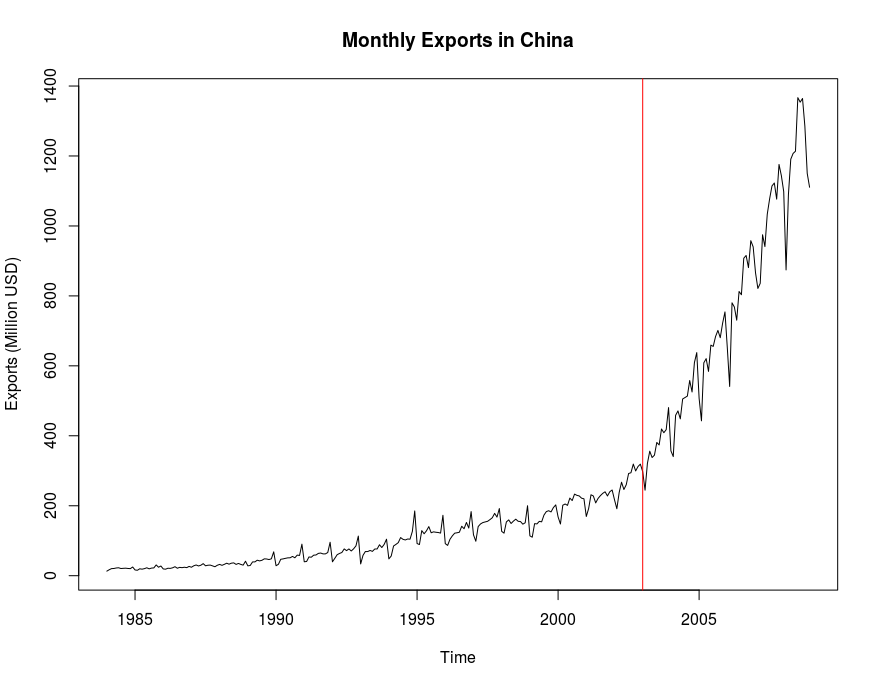
\includegraphics[width=\linewidth]{exports}
\caption{Monthly exports in China}
\label{exports}
\end{minipage}%
\begin{minipage}{.5\textwidth}
\centering
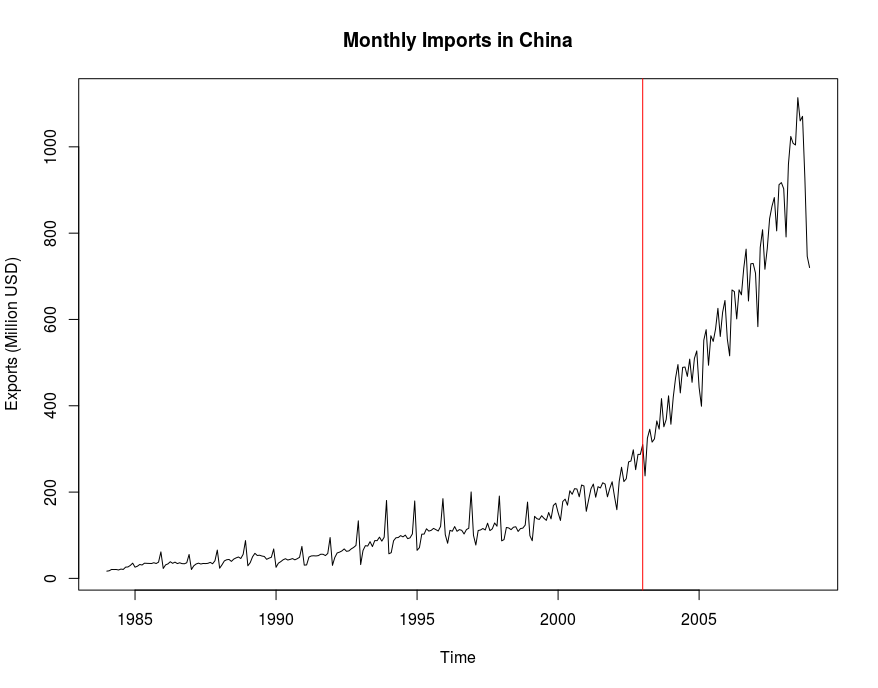
\includegraphics[width=\linewidth]{imports}
\caption{Monthly imports in China}
\label{imports}
\end{minipage}
\end{figure}

The objective is to determine the best model (and parameters) to predict future export figures. In order to be able to perform this testing, we first need to split the data into train and test sets, which we do according to the 80–20 rule. In particular, the data is partitioned in the following way (shown by the vertical line in Figures \ref{exports} and \ref{imports}):

\begin{itemize}
\item Training: January 1984 -- December 2002
\item Test: January 2003 -- December 2008
\end{itemize}

Using this partition, we fit models on the train data up to the end of 2002, and predict export figures for the following 6 years, which we compare to the actual export figures from the test set by computing the predictive root mean squared error (RMSE). To accomplish this task, we use four models:

\begin{itemize}
\item Holt-Winters
\item SARIMA
\item SARIMAX
\item VAR
\end{itemize}

We hope to be able, at the end of this exercise, to determine which model produces the best predictions for this data set, i.e., which model produced the lowest RMSE. This means that the predicted export figures for 2003 -- 2008 were the most similar to the actual export figures in the test data.

Before starting modeling, we first take the log-transform of all the data, seeing as the variance in both exports and imports seem to increase with time. These are shown in Figures \ref{log_exports} and \ref{log_imports}.

\begin{figure}[!ht]
\centering
\begin{minipage}{.5\textwidth}
\centering
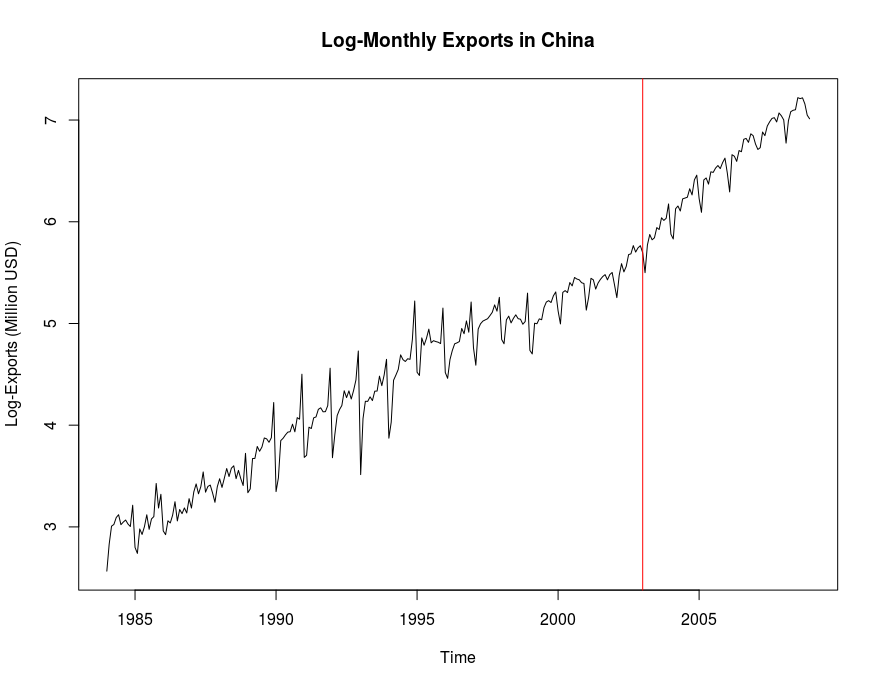
\includegraphics[width=\linewidth]{log_exports}
\caption{Log-Monthly exports in China}
\label{log_exports}
\end{minipage}%
\begin{minipage}{.5\textwidth}
\centering
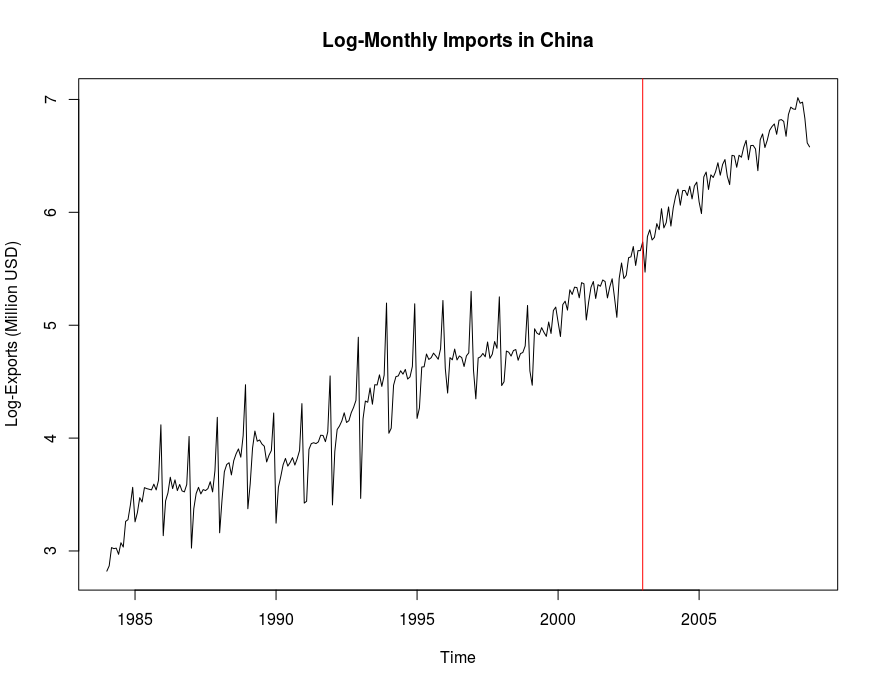
\includegraphics[width=\linewidth]{log_imports}
\caption{Log-Monthly imports in China}
\label{log_imports}
\end{minipage}
\end{figure}

All the R code used is provided at the end of the report.

\newpage
\section{Holt-Winters}
The log-transformed exports data clearly shows trend and seasonality, as seen in Figure \ref{log_exports}. Therefore, we decide to fit an additive Triple Exponential Smoothing Holt-Winters model to the train log-transformed data. We let the \texttt{HoltWinters} function in R determine the smoothing constants $\alpha$, $\beta$, and $\gamma$ to start.

With this model we obtain $\alpha = 0.287$, $\beta = 0.013$, and $\gamma = 0.557$. After completing the steps shown below, we get a test RMSE of $345.0766$ with these constants. Upon further analysis, we reach an optimal set of constants $\alpha = 0.15$, $\beta = 0.5$, and $\gamma = 0.29$. This is the model that we will further analyze.

The model seems to fit the train data reasonably well, as shown in Figure \ref{fit_hw}.

\begin{figure}[!ht]
\centering
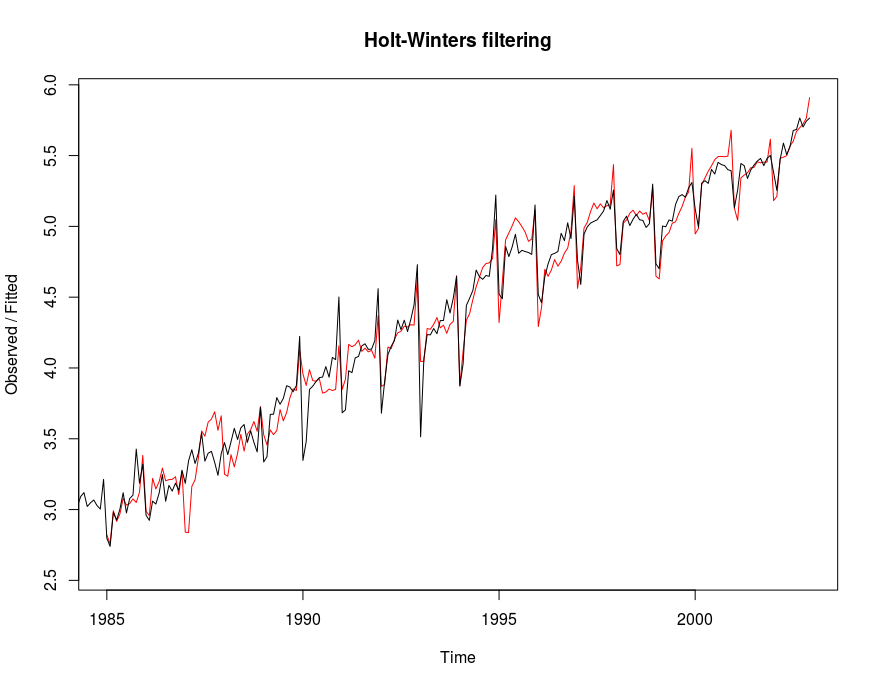
\includegraphics[width=.8\textwidth]{fit_hw}
\caption{Fit of Holt-Winters model on train data}
\label{fit_hw}
\end{figure}

We check the residuals of this model in order to verify that they have zero-mean, are homoskedastic, and are uncorrelated.

This produces the Figures \ref{seq_hw} and \ref{qq_hw}. The first shows that the residuals have approximately zero-mean, seem to be homoskedastic, and seem to be uncorrelated. The QQ-plot has significant skews in both tails, but we assume it's OK. In any case, no disributional assumptions are made for Holt-Winters, so it's not very important.

\begin{figure}[!ht]
\centering
\begin{minipage}{.5\textwidth}
\centering
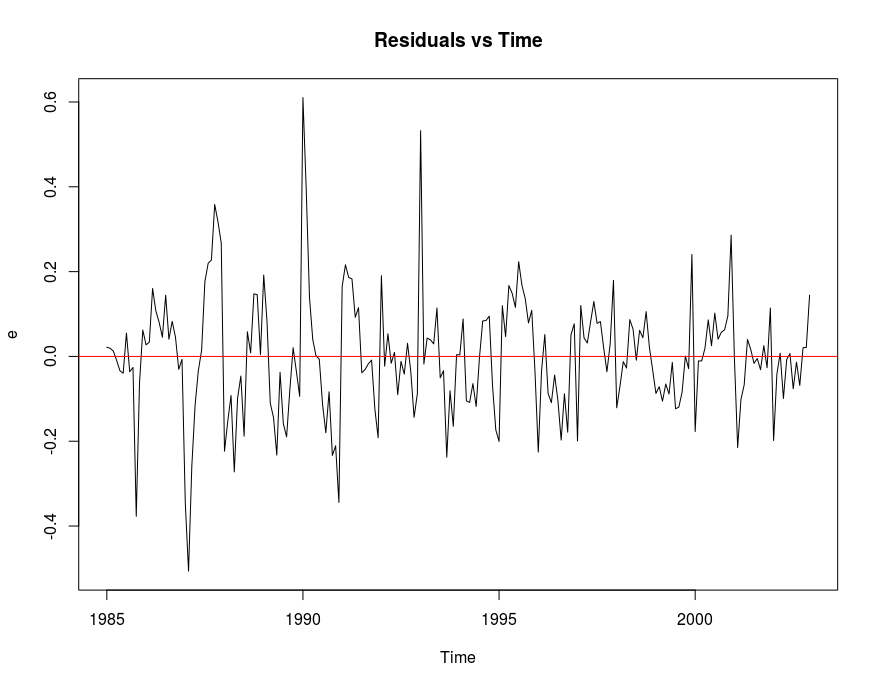
\includegraphics[width=\linewidth]{seq_hw}
\caption{Sequential plot of residuals for Holt-Winters model}
\label{seq_hw}
\end{minipage}%
\begin{minipage}{.5\textwidth}
\centering
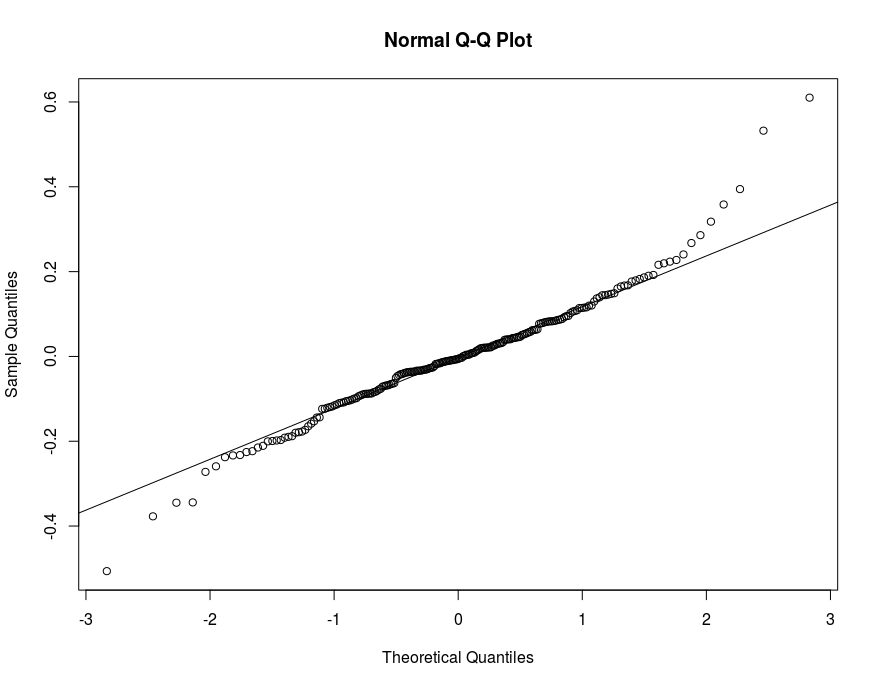
\includegraphics[width=\linewidth]{qq_hw}
\caption{QQ-plot of residuals for Holt-Winters model}
\label{qq_hw}
\end{minipage}
\end{figure}

Forecasting for the six years from 2003 to 2008, this model produces the output shown in Figure \ref{pred_hw}. We can see that our predictions for export data fits closely to the actual values observed (remember, we took the last 20\% of the data set to use for testing). However, the 95\% confidence interval obtained is also very wide, as we are not optimizing to get a low variance $\sigma^2$. 

\begin{figure}[!ht]
\centering
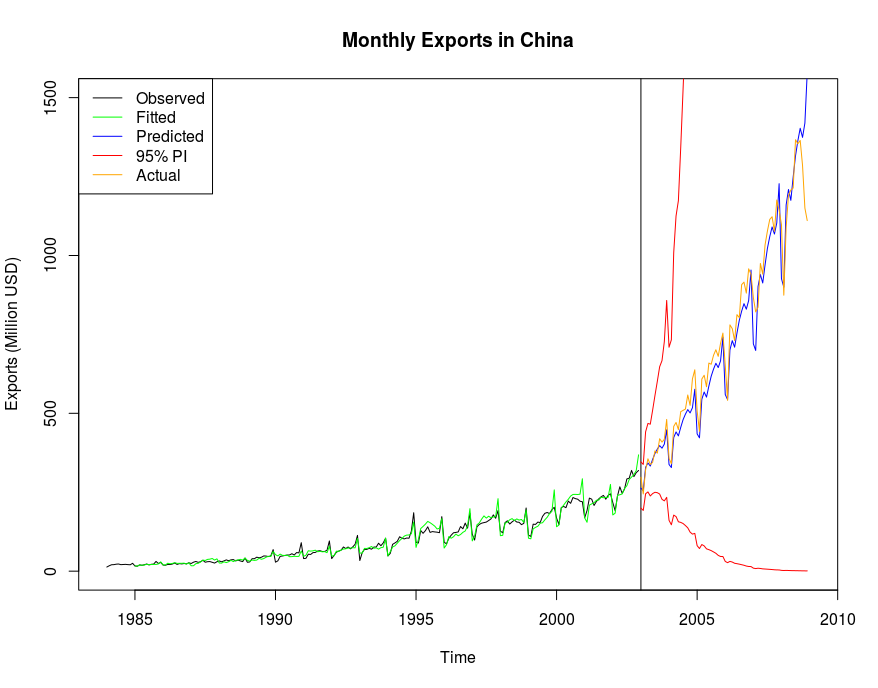
\includegraphics[width=\textwidth]{pred_hw}
\caption{Prediction with Holt-Winters}
\label{pred_hw}
\end{figure}

The values for prediction and 95\% confidence bands are shown in the Table \ref{pred_hw_tab}.

\begin{table}[!ht]
\centering
\resizebox{\textwidth}{!}{\begin{tabular}{c|cccccccccccc}
\textbf{Month} & Jan & Feb & Mar & Apr & May & Jun & Jul & Aug & Sep & Oct & Nov & Dec\\
\hline
\textbf{Prediction} & 262.64 & 255.00 & 328.87 & 342.70 & 332.96 & 353.92 & 372.93 & 386.52 & 397.69 & 389.52 & 402.37 & 447.69\\
\textbf{Lower 95\%} & 199.46 & 192.33 & 245.13 & 250.98 & 238.13 & 245.69 & 249.83 & 248.54 & 244.26 & 227.51 & 222.60 & 233.72\\
\textbf{Upper 95\%} & 345.83 & 338.10 & 441.23 & 467.94 & 465.55 & 509.83 & 556.68 & 601.09 & 647.49 & 666.88 & 727.32 & 857.53\\
\end{tabular}}
\caption{2003 forecast and 95\% confidence interval bands for Holt-Winters}
\label{pred_hw_tab}
\end{table}

For this optimized model, we finally calculate the test RMSE, and obtain a value of $83.92663$. Note: a multiplicative approach was also tested, but led to worse results and is not shown here.

\newpage
\section{SARIMA}
We have already seen that the data shows trend and seasonality. Therefore, we choose to use a SARIMA approach to model the data. We plot the ACF of the log-transformed data to see if we need to difference it. As Figure \ref{acf_sarima} shows exponential decay, we conclude that we need to difference the data for trend. We then plot the ACF again, as shown in Figure \ref{acf1_sarima}, which does not show exponetial decay anymore within periods. However, we see significant spikes at lags multiple of 12, so we need to difference for seasonality, and we use a period of 12. The resulting ACF after this differencing is shown in Figure \ref{acf1.12_sarima}, which seems OK. We plot the trend and seasonally-differenced data to verify that it is stationary, as shown in Figure \ref{exports_1.12}. Therefore, we have $d=1,\ D=1,\ s=12$.

\begin{figure}[!ht]
\centering
\begin{minipage}{.5\textwidth}
\centering
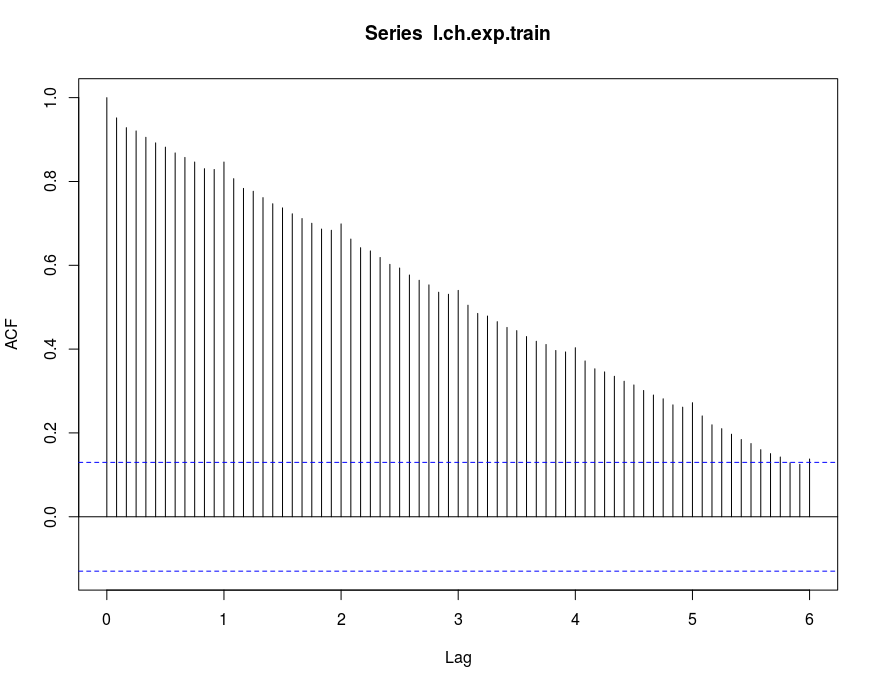
\includegraphics[width=\linewidth]{acf_sarima}
\caption{ACF plot of log-differenced data}
\label{acf_sarima}
\end{minipage}%
\begin{minipage}{.5\textwidth}
\centering
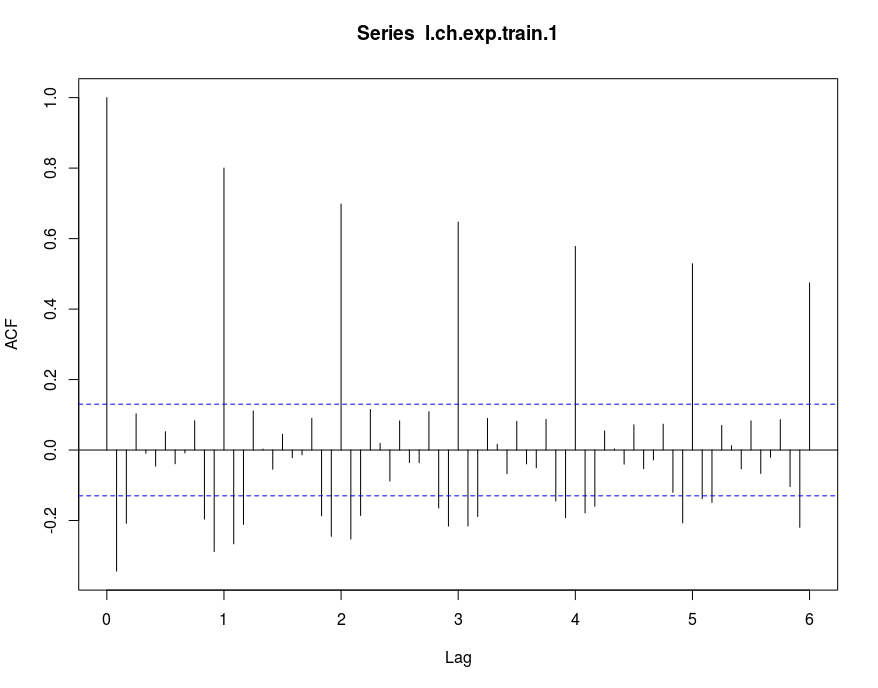
\includegraphics[width=\linewidth]{acf1_sarima}
\caption{ACF plot of trend-differenced data}
\label{acf1_sarima}
\end{minipage}
\end{figure}

\begin{figure}[!ht]
\centering
\begin{minipage}{.5\textwidth}
\centering
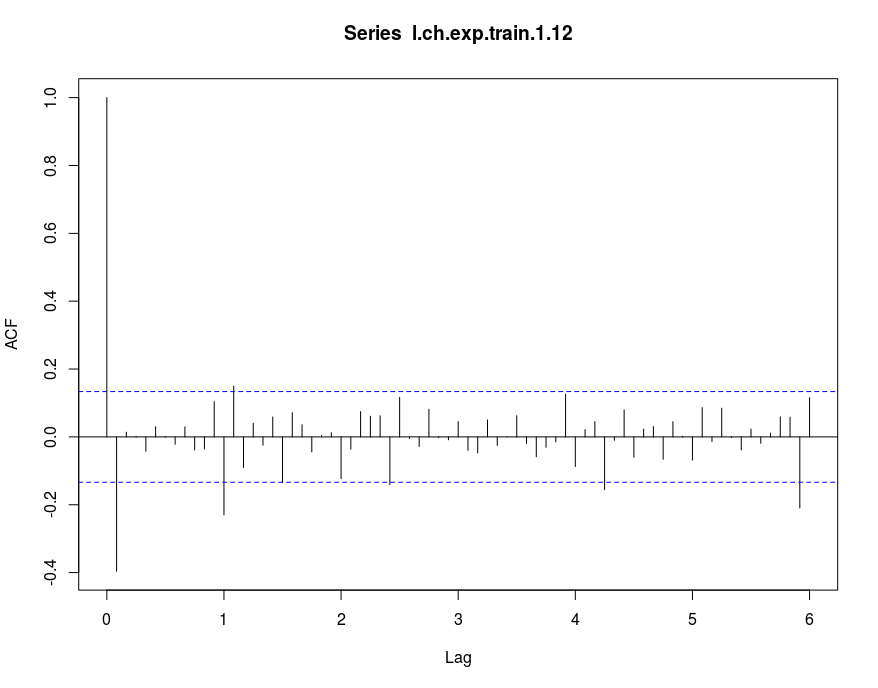
\includegraphics[width=\linewidth]{acf1.12_sarima}
\caption{ACF plot of trend and seasonally-differenced data}
\label{acf1.12_sarima}
\end{minipage}%
\begin{minipage}{.5\textwidth}
\centering
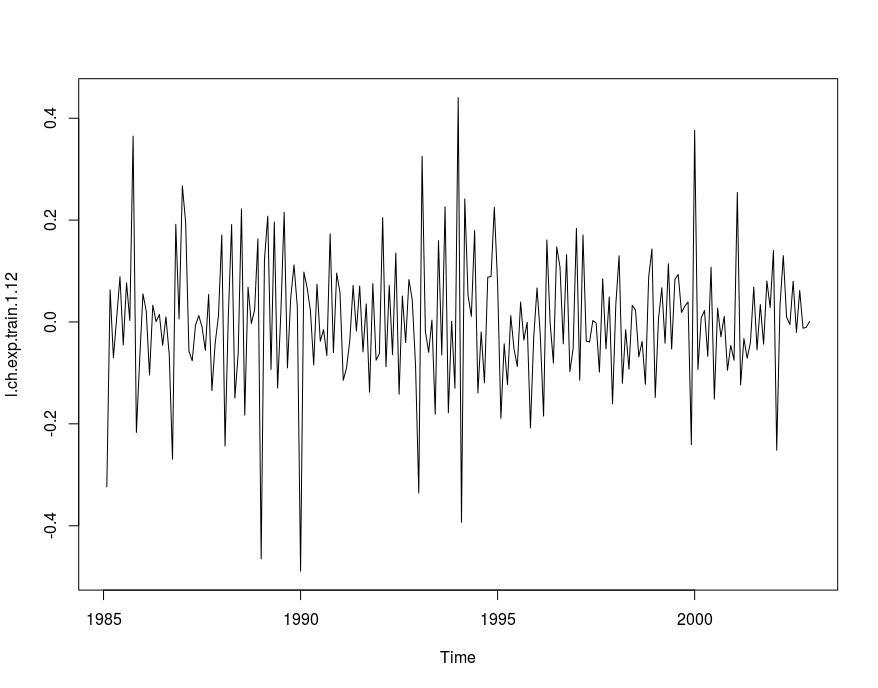
\includegraphics[width=\linewidth]{exports_1.12}
\caption{Trend and seasonally-differenced data}
\label{exports_1.12}
\end{minipage}
\end{figure}

We can now proceed to identify $p,\ q,\ P,\ Q$ from the ACF and PACF plots of this differenced data. From the PACF plot in Figure \ref{acf_pacf_sarima}, we can deduce that $p \leq 2$ and $P \leq 1$. From the ACF plot in Figure \ref{acf_pacf_sarima}, we can deduce that $q \leq 1$ and $Q \leq 1$.

\begin{figure}[!ht]
\centering
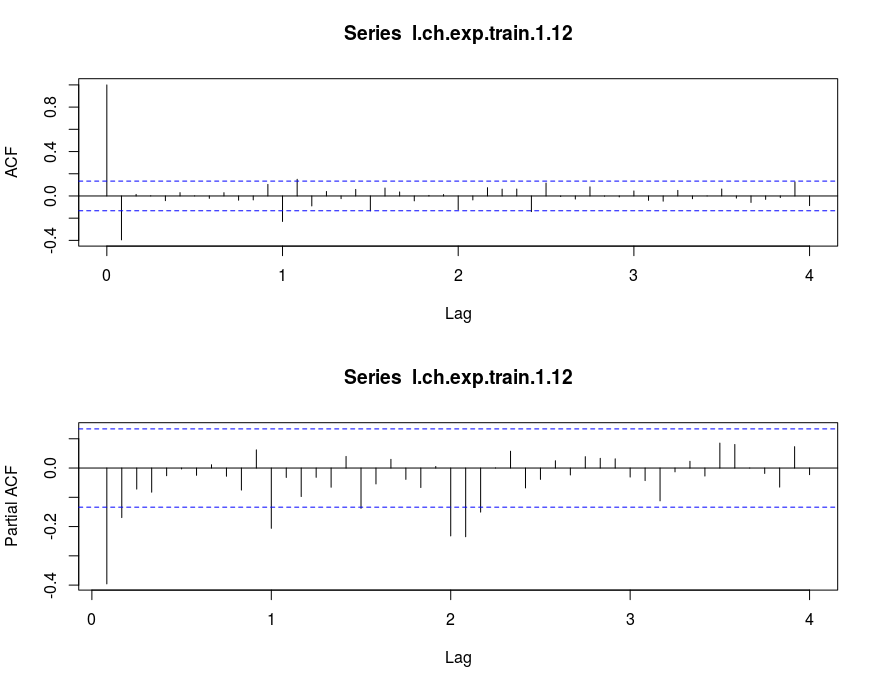
\includegraphics[width=.8\textwidth]{acf_pacf_sarima}
\caption{ACF and PACF plots for trend and seasonally-differenced data}
\label{acf_pacf_sarima}
\end{figure}

After iterating through different models with these values for the parameters, we obtain the optimal SARIMA $(1,1,1)\times(0,1,0)[12]$ model, so the final parameters for this model are $p=1,\ d=1,\ q=1,\ P=0,\ D=1,\ Q=0,\ s=12$.

This model seems to fit the training data pretty well, as shown in Figure \ref{fit_sarima}.

\begin{figure}[!ht]
\centering
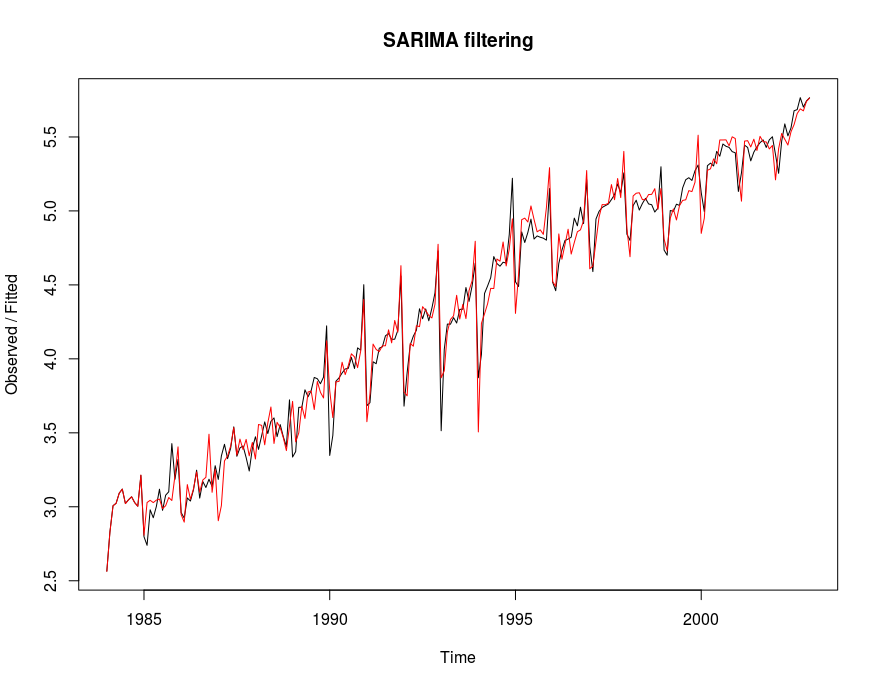
\includegraphics[width=.8\textwidth]{fit_sarima}
\caption{Fit of SARIMA model on training data}
\label{fit_sarima}
\end{figure}

We check the residuals of this model in order to verify that they have zero-mean, are homoskedastic, and are uncorrelated.

This produces the Figures \ref{tsdiag_sarima} and \ref{qq_sarima}. The first shows that the residuals have approximately zero-mean, seem to be homoskedastic, and seem to be uncorrelated (ACF + Ljung-Box test). The QQ-plot has significant skews in both tails, but we assume it's OK.

\begin{figure}[!ht]
\centering
\begin{minipage}{.5\textwidth}
\centering
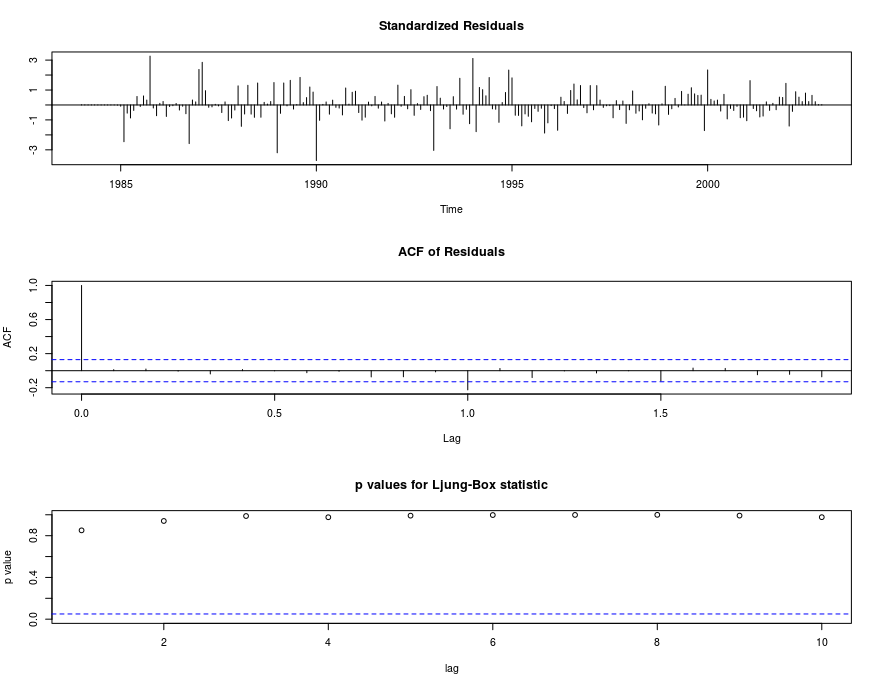
\includegraphics[width=\linewidth]{tsdiag_sarima}
\caption{Residual check plots of residuals for SARIMA model}
\label{tsdiag_sarima}
\end{minipage}%
\begin{minipage}{.5\textwidth}
\centering
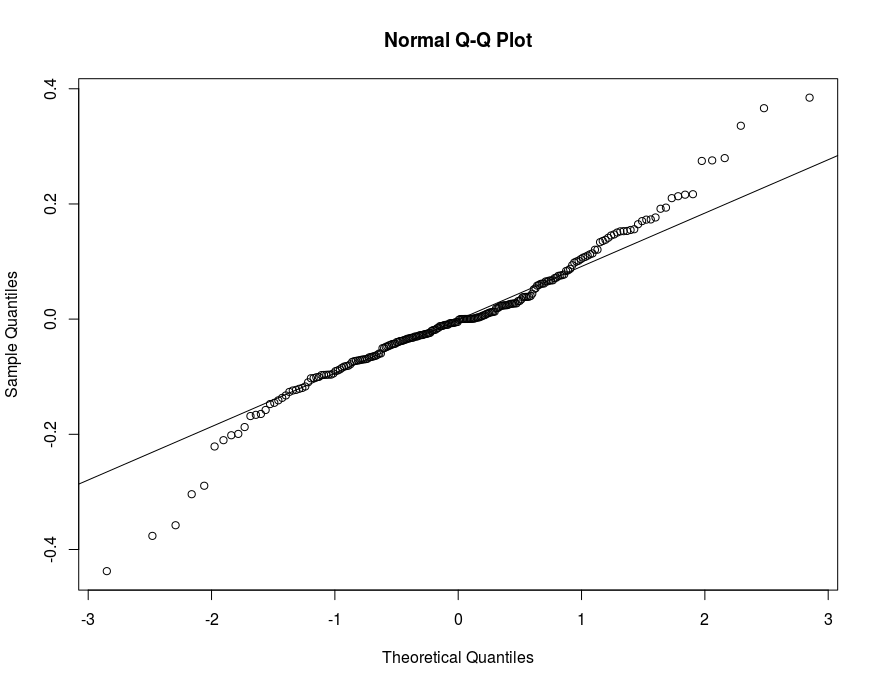
\includegraphics[width=\linewidth]{qq_sarima}
\caption{QQ-plot of residuals for SARIMA model}
\label{qq_sarima}
\end{minipage}
\end{figure}

Forecasting for the six years from 2003 to 2008, this model produces the output shown in Figure \ref{pred_sarima}. We can see that our predictions for export data fits closely to the actual values observed. However, the 95\% confidence interval obtained is also very wide, as we are not optimizing to get a low variance $\sigma^2$. 

\begin{figure}[!ht]
\centering
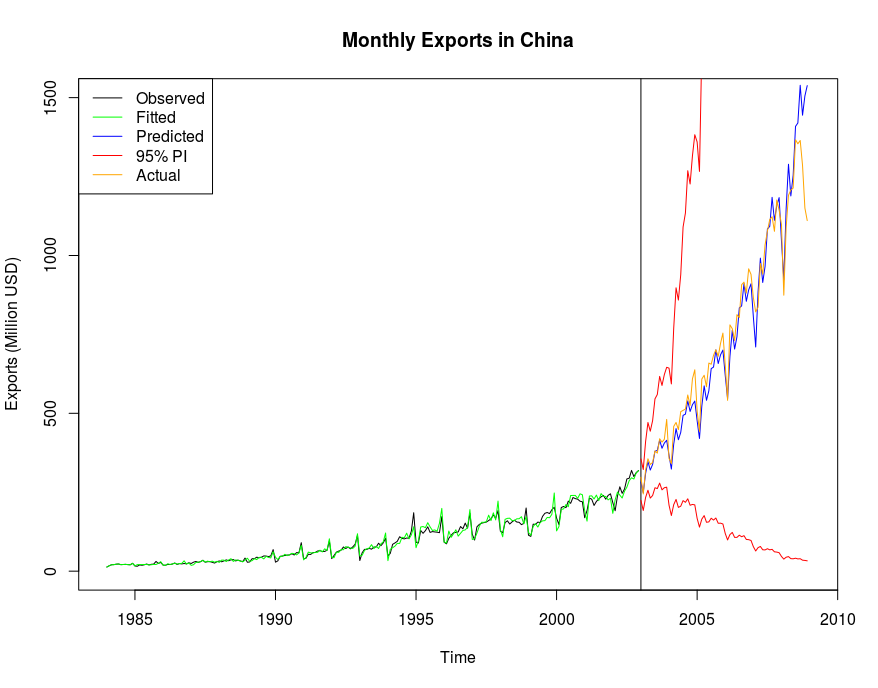
\includegraphics[width=.8\textwidth]{pred_sarima}
\caption{Prediction with SARIMA}
\label{pred_sarima}
\end{figure}

The values for prediction and 95\% confidence bands are shown in the Table \ref{pred_sarima_tab}.

\begin{table}[!ht]
\centering
\resizebox{\textwidth}{!}{\begin{tabular}{c|cccccccccccc}
\textbf{Month} & Jan & Feb & Mar & Apr & May & Jun & Jul & Aug & Sep & Oct & Nov & Dec\\
\hline
\textbf{Prediction} & 282.10 & 248.75 & 309.59 & 347.37 & 320.33 & 338.12 & 379.685 &382.63 & 414.79 & 389.25 & 405.66 & 414.50\\
\textbf{Lower 95\%} & 223.93 & 192.18 & 233.49 & 256.24 & 231.46 & 239.62 & 264.17 & 261.60 & 278.89 & 257.55 & 264.29 & 266.05\\
\textbf{Upper 95\%} & 355.39  & 321.97  & 410.49 &  470.90  & 443.31 &  477.12  & 545.70  & 559.65  & 616.92 &  588.30  & 622.65  & 645.78\\
\end{tabular}}
\caption{2003 forecast and 95\% confidence interval bands for SARIMA}
\label{pred_sarima_tab}
\end{table}

For this optimized model, we finally calculate the test RMSE, and obtain a value of $84.10774$. It performs similarly to the previous Holt-Winters model in prediction.

\newpage
\section{SARIMAX}
We have already defined that the optimal parameters for SARIMA are $p=1,\ d=1,\ q=1,\ P=0,\ D=1,\ Q=0,\ s=12$. We wish to hopefully obtain a better model by including imports as a correlated explanatory variable. Here, we assume that the imports are exogenous, i.e., they influence exports but not the other way around. We therefore create the SARIMAX $(1,1,1)\times(0,1,0)[12]$ model. The fit on the training data is shown in Figure \ref{fit_sarimax}, and it seems to be pretty good.

\begin{figure}[!ht]
\centering
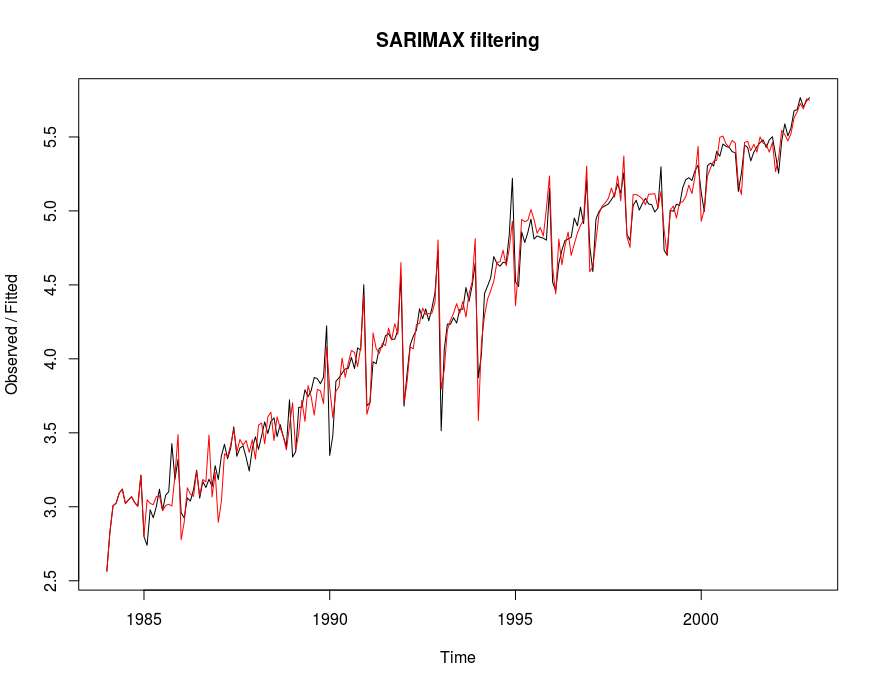
\includegraphics[width=.8\textwidth]{fit_sarimax}
\caption{Fit of SARIMAX model on training data}
\label{fit_sarimax}
\end{figure}

We check the residuals of this model in order to verify that they have zero-mean, are homoskedastic, and are uncorrelated.

This produces the Figures \ref{tsdiag_sarimax} and \ref{qq_sarimax}. The first shows that the residuals have approximately zero-mean, seem to be homoskedastic, and seem to be uncorrelated (ACF + Ljung-Box test). The QQ-plot has significant skews in both tails, but we assume it's OK.

\begin{figure}[!ht]
\centering
\begin{minipage}{.5\textwidth}
\centering
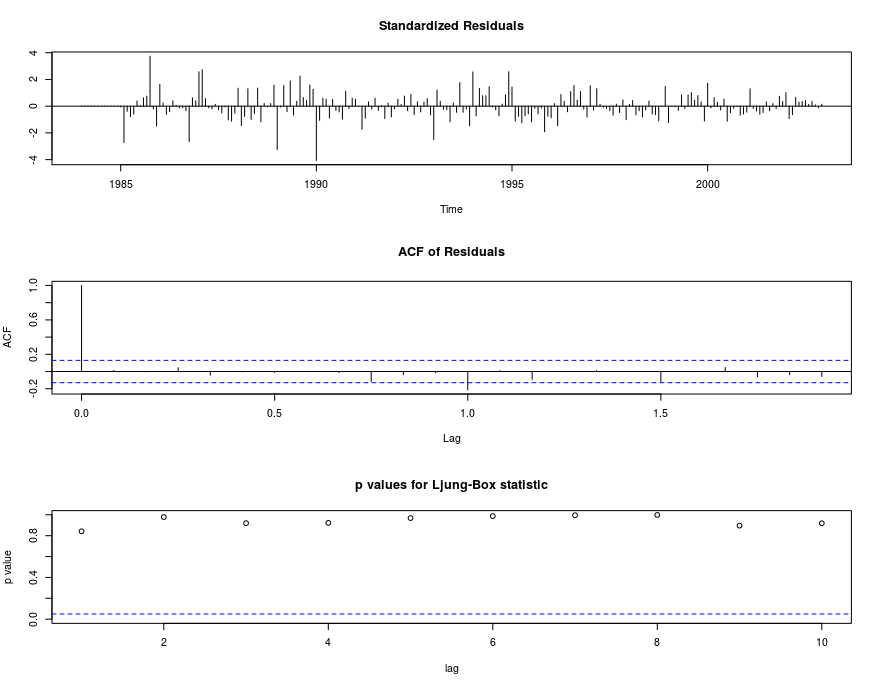
\includegraphics[width=\linewidth]{tsdiag_sarimax}
\caption{Residual check plots of residuals for SARIMAX model}
\label{tsdiag_sarimax}
\end{minipage}%
\begin{minipage}{.5\textwidth}
\centering
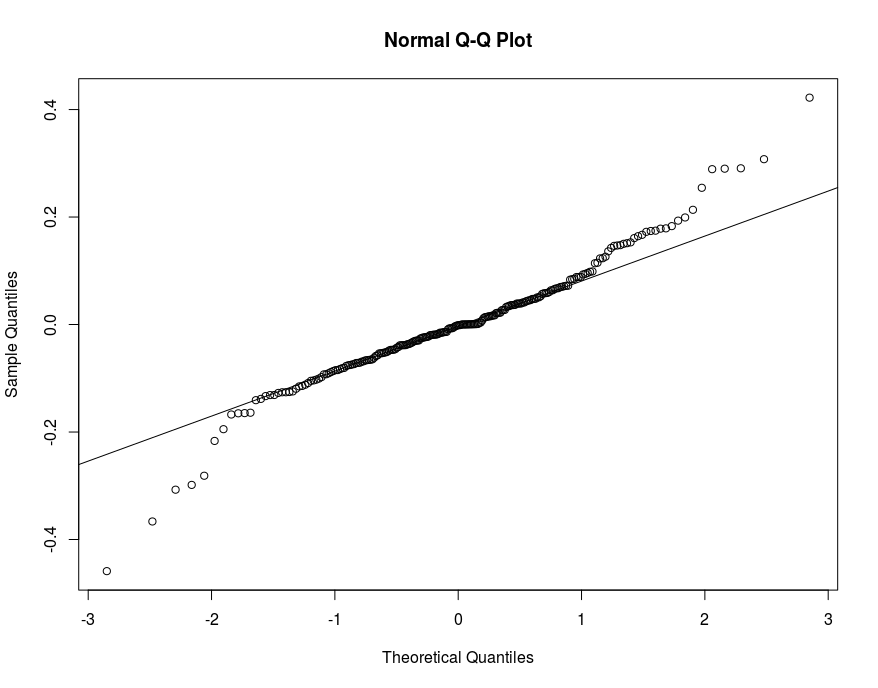
\includegraphics[width=\linewidth]{qq_sarimax}
\caption{QQ-plot of residuals for SARIMAX model}
\label{qq_sarimax}
\end{minipage}
\end{figure}

Forecasting for the six years from 2003 to 2008, this model produces the output shown in Figure \ref{pred_sarimax}. We can see that our predictions for export data fits closely to the actual values observed. However, the 95\% confidence interval obtained is also very wide, as we are not optimizing to get a low variance $\sigma^2$. 

\begin{figure}[!ht]
\centering
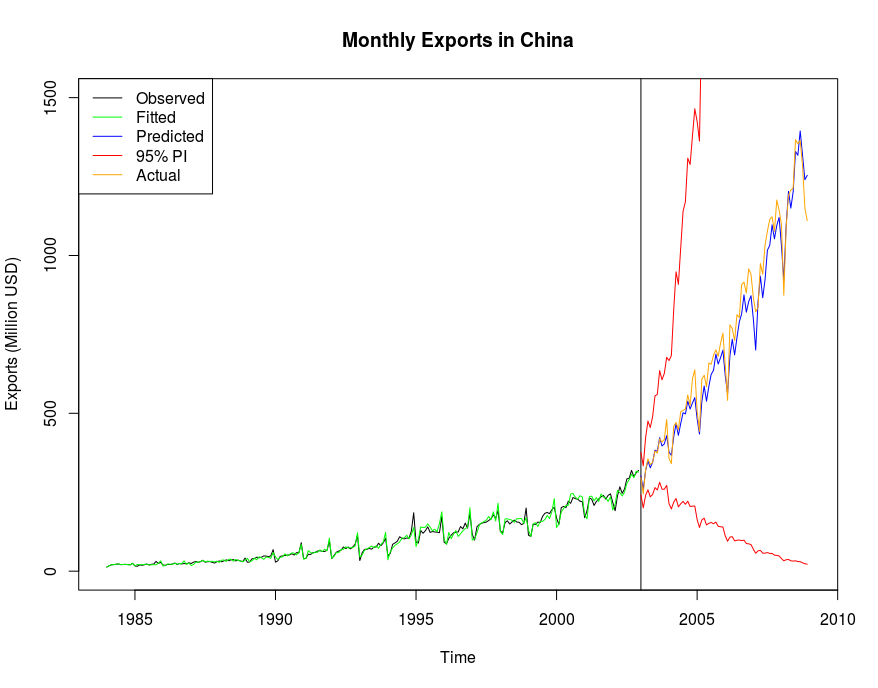
\includegraphics[width=.8\textwidth]{pred_sarimax}
\caption{Prediction with SARIMAX}
\label{pred_sarimax}
\end{figure}

The values for prediction and 95\% confidence bands are shown in the Table \ref{pred_sarimax_tab}.

\begin{table}[!ht]
\centering
\resizebox{\textwidth}{!}{\begin{tabular}{c|cccccccccccc}
\textbf{Month} & Jan & Feb & Mar & Apr & May & Jun & Jul & Aug & Sep & Oct & Nov & Dec\\
\hline
\textbf{Prediction} & 301.26 & 258.51 & 318.74 & 349.92 & 327.24 & 344.85 & 383.31 & 379.39 & 422.88 & 396.54 & 403.15 & 429.05\\
\textbf{Lower 95\%} & 241.52 & 200.29 & 240.38 & 257.54 & 235.47 & 242.95 & 264.72 & 257.11 & 281.46 & 259.41 & 259.40 & 271.69\\
\textbf{Upper 95\%} & 375.77 &  333.65  & 422.64  & 475.44 &  454.78 &  489.49  & 555.03 &  559.83  & 635.34 &  606.14 &  626.55  & 677.56\\
\end{tabular}}
\caption{2003 forecast and 95\% confidence interval bands for SARIMAX}
\label{pred_sarimax_tab}
\end{table}

For this optimized model, we finally calculate the test RMSE, and obtain a value of $52.09312$. It performs significantly better than both previous models we've seen. Adding imports as an exogenous explanatory variable helped make predictions better.

\newpage
\section{VAR}
Finally, we want to see whether imports can be thought of as an endogenous explanatory variable, i.e., it has an effect on exports and vice-versa. For this, we build a VAR model. We use the \texttt{VARselect} function in R to help us determine the order $p$ of the model. Using BIC as the selection criteria, we decide to try $p = 3$. This is also a parcimonious choice, seeing as AIC selects an optimal order of 10, which would make the model considerably more complicated. Therefore, we create the VAR(3) model with trend and seasonality of 12. 

Using this VAR(3) model, we get two equations (one per variable, i.e., one for exports and one for imports). The fit as well as ACF and PACF plots are shown in Figures \ref{fit_var_exp} and \ref{fit_var_imp}. Both fits seem to be good, and the residuals have zero-mean, seem fairly homoskedastic, but the ACF and PACF plots of the residuals show seasonal correlations (which is expected since we didn't difference the data). No distributional assumptions are made for this approach, so we don't need to check for normality.

\begin{figure}[!ht]
\centering
\begin{minipage}{.5\textwidth}
\centering
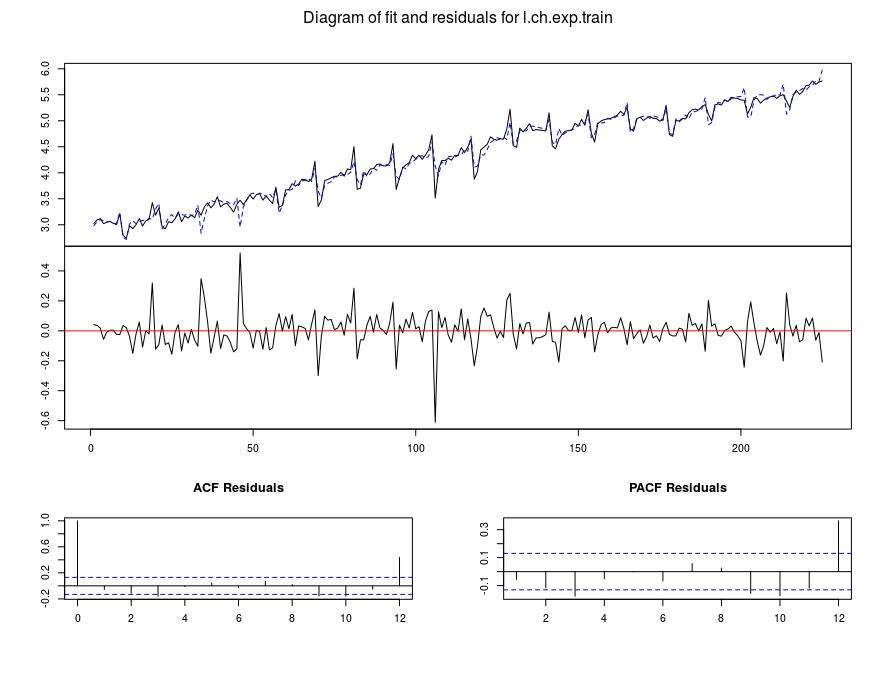
\includegraphics[width=\linewidth]{fit_var_exp}
\caption{Fit of VAR(3) model on exports}
\label{fit_var_exp}
\end{minipage}%
\begin{minipage}{.5\textwidth}
\centering
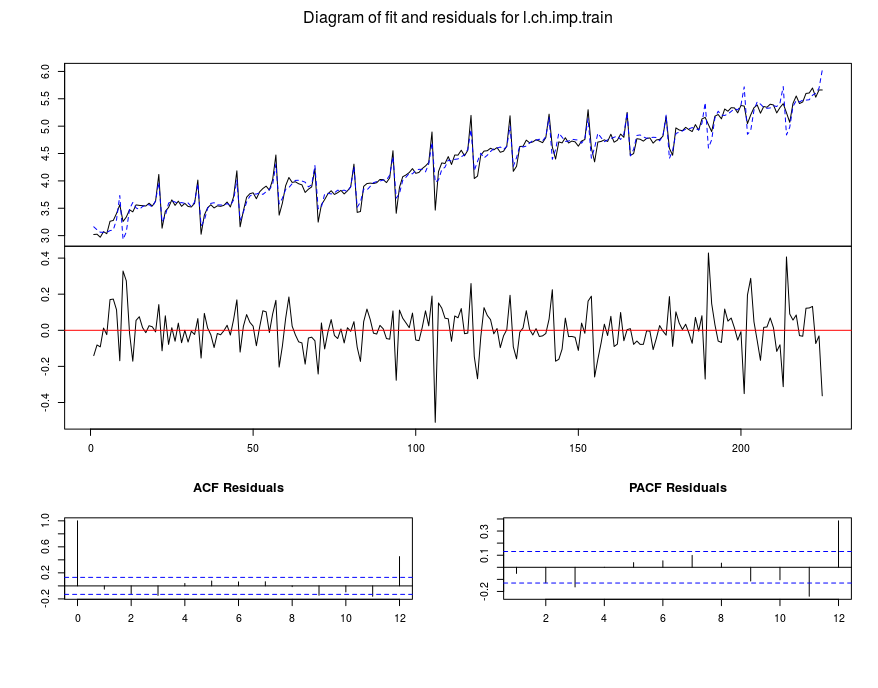
\includegraphics[width=\linewidth]{fit_var_imp}
\caption{Fit of VAR(3) model on imports}
\label{fit_var_imp}
\end{minipage}
\end{figure}

Forecasting for the six years from 2003 to 2008, this model produces the output shown in Figure \ref{pred_var}. We can see that our predictions for export data does not fit as closely to the actual values observed as previous models. However, they are within the 95\% confidence interval obtained, so it is not too bad a model.

\begin{figure}[!ht]
\centering
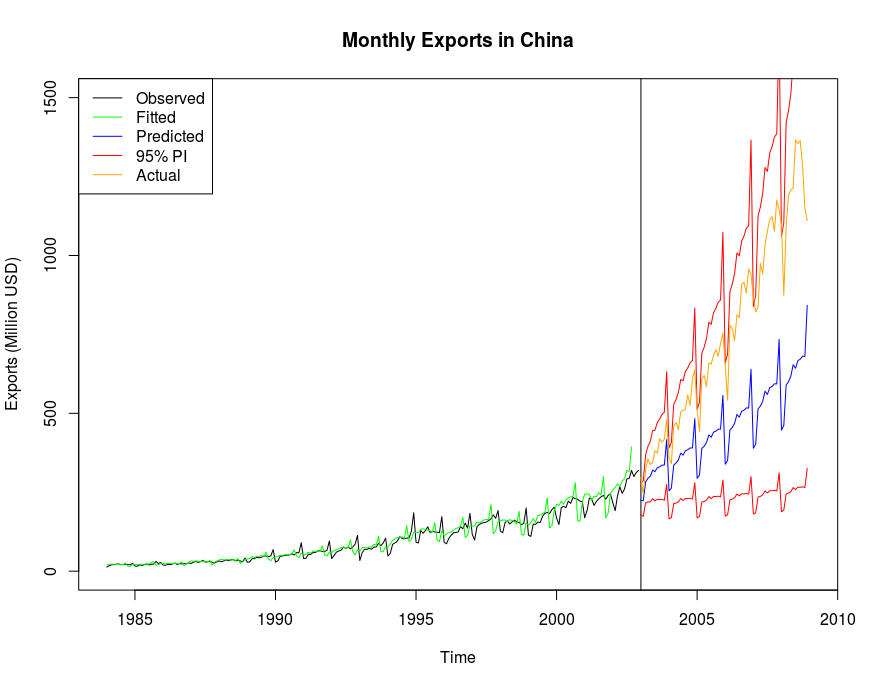
\includegraphics[width=.8\textwidth]{pred_var}
\caption{Prediction with VAR(3)}
\label{pred_var}
\end{figure}

In addition, predictions for both variables (exports and imports) are shown in Figure \ref{pred_var2}. Note however that these two plots are shown on the log-transformed data.

\begin{figure}[!ht]
\centering
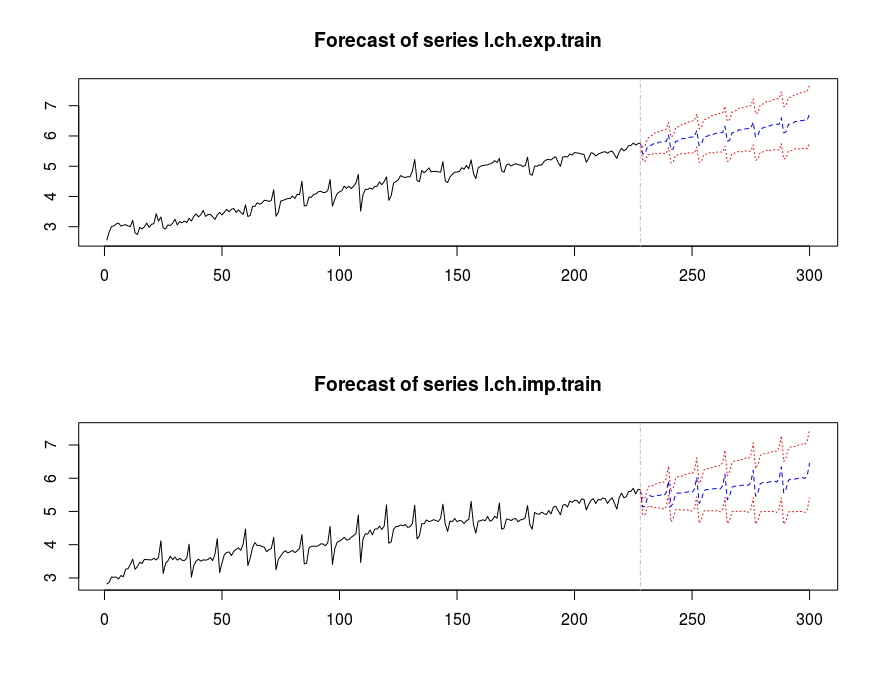
\includegraphics[width=.8\textwidth]{pred_var2}
\caption{Prediction with VAR(3) for export and import (log-transformed)}
\label{pred_var2}
\end{figure}

The values for prediction and 95\% confidence bands are shown in the Table \ref{pred_var_tab}.

\begin{table}[!ht]
\centering
\resizebox{\textwidth}{!}{\begin{tabular}{c|cccccccccccc}
\textbf{Month} & Jan & Feb & Mar & Apr & May & Jun & Jul & Aug & Sep & Oct & Nov & Dec\\
\hline
\textbf{Prediction} & 224.04 & 222.97 & 282.31 & 294.36 & 300.36 & 319.65 & 315.36 & 327.52 & 330.60 & 335.97 & 336.19 & 416.76\\
\textbf{Lower 95\%} & 179.18 & 173.77 & 216.11 & 219.18 & 219.48 & 229.60 & 222.77 & 227.88 & 226.75 & 227.31 & 224.52 & 274.85\\
\textbf{Upper 95\%} & 280.12 &  286.11 &  368.78 &  395.34 &  411.05 &  445.03 &  446.45 &  470.73 &  482.02 &  496.56 &  503.40 &  631.92\\
\end{tabular}}
\caption{2003 forecast and 95\% confidence interval bands for VAR}
\label{pred_var_tab}
\end{table}

For this optimized model, we finally calculate the test RMSE, and obtain a value of $351.1797$. It performs significantly worse than all previous models we've seen. Adding imports as an endogenous explanatory variable did not help make predictions better, and in fact made them much worse.

\newpage
\section{Conclusion}
In this assignment, we set out to use several distinct approaches in order to best generate prediction of future export figures for China. We tried a triple exponential smoothing with Holt-Winters, a SARIMA model, a SARIMAX model with import figures as an exogenous variable, and finally a VAR(3) model with import figures as an endogenous variable. Their performace was assessed through test RMSE on the final 20\% of the data, i.e., from January 2003 to December 2008. These are summarized in Table \ref{rmse}, where we can recall that our SARIMAX $(1,1,1)\times(0,1,0)[12]$ produced the lowest RMSE and therefore generated the closest predictions to reality. From this result, we can say that import figures are an exogneous explanatory variable, meaning that they influence exports, but not the other way around.

\begin{table}[!ht]
\centering
\begin{tabular}{c|cccc}
\textbf{Model} & Holt-Winters & SARIMA & SARIMAX & VAR\\
\hline
\textbf{RMSE} & 83.92663 & 84.10774 & 52.09312 & 351.1797 \\
\end{tabular}
\caption{Summary of test RMSE for the four approaches seen in this report (lower is better)}
\label{rmse}
\end{table}

\newpage
\section{R Code}
\color{blue}
\begin{Verbatim}[frame=single]
# Reset R session
rm(list=ls())
cat("\014")

# Load libraries
library(tseries)
library(forecast)
library(lawstat)
library(vars)

#######################################
##### IMPORT DATA, VISUALIZE
#######################################
china <- read.csv("china.csv")
ch.exp <- ts(china$ch.exp, start = c(1984,1), frequency = 12)
ch.imp <- ts(china$ch.imp, start = c(1984,1), frequency = 12)

# train and test files (80/20)
ch.exp.train <- ts(ch.exp[time(ch.exp) < 2003], start = c(1984,1), frequency = 12)
ch.exp.test <- ts(ch.exp[time(ch.exp) >= 2003], start = c(2003,1), frequency = 12)
ch.imp.train <- ts(ch.imp[time(ch.imp) < 2003], start = c(1984,1), frequency = 12)
ch.imp.test <- ts(ch.imp[time(ch.imp) >= 2003], start = c(2003,1), frequency = 12)

plot(ch.exp.train, main = "Monthly Exports in China", ylab = "Exports (Million USD)",
     xlab = "Time") # trend + seasonality -> log-transform
plot(log(ch.exp.train), main = "Log-Monthly Exports in China",
     ylab = "Log-Exports (Million USD)", xlab = "Time")

plot(ch.exp, main = "Monthly Exports in China", ylab = "Exports (Million USD)",
     xlab = "Time")
abline(v=2003, col="red")
plot(ch.imp, main = "Monthly Imports in China", ylab = "Exports (Million USD)",
     xlab = "Time")
abline(v=2003, col="red")

l.ch.exp <- log(ch.exp)
l.ch.imp <- log(ch.imp)
l.ch.exp.train <- log(ch.exp.train)
l.ch.exp.test <- log(ch.exp.test)
l.ch.imp.train <- log(ch.imp.train)
l.ch.imp.test <- log(ch.imp.test)

plot(l.ch.exp, main = "Log-Monthly Exports in China",
     ylab = "Log-Exports (Million USD)", xlab = "Time")
abline(v=2003, col="red")
plot(l.ch.imp, main = "Log-Monthly Imports in China",
     ylab = "Log-Exports (Million USD)", xlab = "Time")
abline(v=2003, col="red")

#######################################
##### HOLT-WINTERS
#######################################
par(mfrow = c(1,1))
plot(l.ch.exp.train, main = "Monthly Exports in China", ylab = "Exports (Million USD)",
     xlab = "Time")
m.hw <- HoltWinters(x = l.ch.exp.train, seasonal = "add", alpha=.15, beta=.5, gamma=.29)
#m.hw$alpha #0.2865475 
#m.hw$beta #0.01290944 
#m.hw$gamma #0.5566387 
plot(m.hw)
#plot(forecast(m.hw, h = 72))
#points(l.ch.exp.test, type = "l", col = "green")

#summary(m.hw)

# Check residuals
e <- m.hw$fitted[,1] - l.ch.exp.train
plot(e, main="Residuals vs Time")
abline(h=0, col="red")
qqnorm(e)
qqline(e)

# Forecasting
f <- forecast(m.hw, h=72, level=0.95)
l <- ts(f$lower, start = c(2003, 1), frequency = 12)  #95% PI LL
h <- ts(f$upper, start = c(2003, 1), frequency = 12) #95% PI UL
pred <- f$mean #predictions
par(mfrow=c(1,1))
plot(ch.exp.train, xlim=c(1984, 2009), ylim=c(0, 1500), main = "Monthly Exports in China",
     ylab = "Exports (Million USD)", xlab = "Time")
abline(v = 2003, lwd = 1, col = "black")
points(exp(pred), type = "l", col = "blue")
points(exp(l), type = "l", col = "red")
points(exp(h), type = "l", col = "red")
points(exp(f$fitted), type="l", col = "green")
points(ch.exp.test, type = "l", col = "orange")
legend("topleft", legend = c("Observed", "Fitted", "Predicted", "95% PI", "Actual"),
       lty = 1, col = c("black", "green", "blue", "red", "orange"), cex = 1)

# Test RMSE
pred.hw <- pred
rmse.hw <- sqrt(mean((ch.exp.test - exp(pred.hw))^2))
rmse.hw

#######################################
##### SARIMA
#######################################
plot(l.ch.exp.train, main = "Log-Monthly Exports in China", 
     ylab = "Log-Exports (Million USD)", xlab = "Time")
acf(l.ch.exp.train, lag.max = 72)
adf.test(l.ch.exp.train) #need to difference
l.ch.exp.train.1 = diff(l.ch.exp.train)
acf(l.ch.exp.train.1, lag.max = 72)
adf.test(l.ch.exp.train.1) #stop -> d=1
#ndiffs(x=ch.exp.train, test="adf", max.d=10)
# difference for season with s=12
l.ch.exp.train.1.12 = diff(l.ch.exp.train.1, lag = 12)
acf(l.ch.exp.train.1.12, lag.max = 72)
#nsdiffs(ch.exp.train.1, 12)

# this looks good. d=1, D=1, s=12
par(mfrow=c(2,1))
acf(l.ch.exp.train.1.12, lag.max = 48) #q<=1, Q<=1
pacf(l.ch.exp.train.1.12, lag.max = 48) #p<=2, P<=1

# create SARIMA (1,1,1)x(0,1,0)[12]
m <- arima(l.ch.exp.train, order = c(1,1,1), seasonal = list(order = c(0,1,0), period = 12))

# Plot fitted values over the data
par(mfrow=c(1,1))
plot(l.ch.exp.train, main = "SARIMA filtering", 
     ylab = "Observed / Fitted", xlab = "Time")
fit <- l.ch.exp.train-m$residuals
lines(fit, col="red")

summary(m)
#auto.arima(l.ch.exp.train, allowdrift = F)

# Check assumptions of model
par(mfrow=c(1,1))
tsdiag(m)
qqnorm(m$residuals)
qqline(m$residuals)

# Forecasting
f <- forecast(m, h=72, level=0.95)
l <- ts(f$lower, start = c(2003, 1), frequency = 12)  #95% PI LL
h <- ts(f$upper, start = c(2003, 1), frequency = 12) #95% PI UL
pred <- f$mean #predictions
par(mfrow=c(1,1))
plot(ch.exp.train, xlim=c(1984,2009), ylim=c(0,1500), main = "Monthly Exports in China",
     ylab = "Exports (Million USD)", xlab = "Time")
abline(v = 2003, lwd = 1, col = "black")
points(exp(pred), type = "l", col = "blue")
points(exp(l), type = "l", col = "red")
points(exp(h), type = "l", col = "red")
points(exp(f$fitted), type="l", col = "green")
points(ch.exp.test, type = "l", col = "orange")
legend("topleft", legend = c("Observed", "Fitted", "Predicted", "95% PI", "Actual"),
       lty = 1, col = c("black", "green", "blue", "red", "orange"), cex = 1)

# Test RMSE
pred.sarima <- pred
rmse.sarima <- sqrt(mean((ch.exp.test - exp(pred.sarima))^2))
rmse.sarima

#######################################
##### SARIMAX
#######################################
# create SARIMAX (1,1,1)x(0,1,0)[12]
m.x <- arima(l.ch.exp.train, order = c(1,1,1), seasonal = list(order = c(0,1,0),
                                                               period = 12),
             xreg = data.frame(l.ch.imp.train))

# Plot fitted values over the data
par(mfrow=c(1,1))
plot(l.ch.exp.train, main = "SARIMAX filtering", 
     ylab = "Observed / Fitted", xlab = "Time")
fit <- l.ch.exp.train-m.x$residuals
lines(fit, col="red")

summary(m.x)

# Check assumptions of model
par(mfrow=c(1,1))
tsdiag(m.x)
qqnorm(m.x$residuals)
qqline(m.x$residuals)

# Forecasting
f <- forecast(m.x, h=72, level=0.95, xreg = data.frame(l.ch.imp.test))
l <- ts(f$lower, start = c(2003, 1), frequency = 12)  #95% PI LL
h <- ts(f$upper, start = c(2003, 1), frequency = 12) #95% PI UL
pred <- f$mean #predictions
par(mfrow=c(1,1))
plot(ch.exp.train, xlim=c(1984,2009), ylim=c(0,1500), main = "Monthly Exports in China",
     ylab = "Exports (Million USD)", xlab = "Time")
abline(v = 2003, lwd = 1, col = "black")
points(exp(pred), type = "l", col = "blue")
points(exp(l), type = "l", col = "red")
points(exp(h), type = "l", col = "red")
points(exp(f$fitted), type="l", col = "green")
points(ch.exp.test, type = "l", col = "orange")
legend("topleft", legend = c("Observed", "Fitted", "Predicted", "95% PI", "Actual"),
       lty = 1, col = c("black", "green", "blue", "red", "orange"), cex = 1)

# Test RMSE
pred.sarimax <- pred
rmse.sarimax <- sqrt(mean((ch.exp.test - exp(pred.sarimax))^2))
rmse.sarimax

#######################################
##### VAR
#######################################
VARselect(y = data.frame(l.ch.exp.train, l.ch.imp.train)) #p=3

# For the sake of parsimony let's choose p=2
m.var <- VAR(y = data.frame(l.ch.exp.train, l.ch.imp.train), p = 3, season = 12,
             type = "trend")
plot(m.var)

summary(m.var)

# Let's now do some forecasting with this model
pred <- predict(m.var, n.ahead = 72, ci = 0.95)
plot(pred)

# Forecasting
f <- ts(pred$fcst$l.ch.exp.train[,1], start = c(2003, 1), frequency = 12)
l <- ts(pred$fcst$l.ch.exp.train[,2], start = c(2003, 1), frequency = 12)  #95% PI LL
h <- ts(pred$fcst$l.ch.exp.train[,3], start = c(2003, 1), frequency = 12) #95% PI UL
pred_ <- ts(m.var$varresult$l.ch.exp.train$fitted.values, start = c(1984,1), frequency = 12)
par(mfrow=c(1,1))
plot(ch.exp.train, xlim=c(1984,2009), ylim=c(0,1500), main = "Monthly Exports in China",
     ylab = "Exports (Million USD)", xlab = "Time")
abline(v = 2003, lwd = 1, col = "black")
points(exp(f), type = "l", col = "blue")
points(exp(l), type = "l", col = "red")
points(exp(h), type = "l", col = "red")
points(exp(pred_), type="l", col = "green")
points(ch.exp.test, type = "l", col = "orange")
legend("topleft", legend = c("Observed", "Fitted", "Predicted", "95% PI", "Actual"),
       lty = 1, col = c("black", "green", "blue", "red", "orange"), cex = 1)

# Test RMSE
pred.var <- pred$fcst$l.ch.exp.train[,1]
rmse.var <- sqrt(mean((ch.exp.test - exp(pred.var))^2))
rmse.var

\end{Verbatim}

\end{document}
